%\documentclass[12pt]{article}
%\usepackage[a4paper, margin=1in]{geometry} 
%\usepackage{graphicx} 
%\usepackage{hyperref}
%\usepackage{float}
%\usepackage{multicol}
%\usepackage{multirow}
%\usepackage{amsmath}
%\usepackage[font=small, labelfont=bf]{caption}
%
%\begin{document}

%
% Sequence profiles 
%
\subsection{Sequence profiles}
A protein sequence profile is a two-dimensional array that contains position-specific scores.

%
% Profile values
%
\subsubsection*{Profile values}
A profile is based on position-specific weights and a score matrix. \\ \\

$\begin{aligned}
\mathrm{Prof}_{ra} :& \text{ Position-specific score of } a \text{ at position } r \\ \\
R_{ab} :& \text{ Pair-wise score of } a \text{ and } b \\
r :& \text{ Position in MSA}  \\
a, b :& \text{ Nucleotide/amino acid element}  \\
M :& \text{ All nucleotides/amino acids}  \\ \\
W_{rb} :& \text{ Weight value of }  b \text{ at position } r 
\end{aligned} $

%
% Profile with linear weights
%
\subsubsection*{Profile with linear weights}

\bigskip 

$\begin{aligned}
\mathrm{Prof}_{ra} =& \dfrac{1}{m_r} \sum_{b \in M}{} R_{ba} F_{rb} \\ \\
W_{rb} =& \dfrac{F_{rb}}{m_{r}} \\
F_{rb} :& \text{ The number of occurrences of } b \text{ at position }  r \\
m_{r} :& \text{ The number of residues without gaps at position } r 
\end{aligned} $

%
% Example of profile with linear weights
%
\subsubsection*{Example of profile with linear weights}

Make a profile with linear weights. \\

\noindent
Alignment
\begin{verbatim}
   Seq1 AGC
   Seq2 -AC
   Seq3 AAT
\end{verbatim}

\medskip 

\noindent
Scoring matrix
\begin{table}[H]
\centering
\small
\begin{tabular}{|c|c|c|c|c|}
\hline
  & A  & G  & C  & T  \\ \hline
A & 2  & 1  & -3 & -2 \\ \hline
G & 1  & 3  & -2 & -1 \\ \hline
C & -3 & -2 & 4  & 1  \\ \hline
T & -2 & -1 & 1  & 2  \\ \hline
\end{tabular}
\end{table}

\noindent
Scores can be calculated as follows. \\

$\begin{aligned}
\mathrm{A1}: & \quad 1/2 \times (2 \times 2 + 1 \times 0 + (-3) \times 0 + (-2) \times 0) = 1/2 \times 4 = 2 \\
\mathrm{G1}: & \quad 1/2 \times (1 \times 2 + 3 \times 0 + (-2) \times 0 + (-1) \times 0) = 1/2 \times 2 = 1 \\
\mathrm{C1}: & \quad 1/2 \times ((-3) \times 2 + (-2) \times 0 + 4 \times 0 + 1 \times 0) = 1/2 \times (-6) = -3 \\
\mathrm{T1}: & \quad 1/2 \times ((-2) \times 2 + (-1) \times 0 + 1 \times 0 + 2 \times 0) = 1/2 \times (-4) = -2 \\ \\
\mathrm{A2}: & \quad 1/3 \times (2 \times 2 + 1 \times 1+(-3) \times 0+(-2) \times 0) = 1/3 \times 5=1.67 \\
\mathrm{G2}: & \quad 1/3 \times (1 \times 2 + 3 \times 1+(-2) \times 0+(-1) \times 0) = 1/3 \times 5=1.67 \\
\mathrm{C2}: & \quad 1/3 \times ((-3) \times 2 + (-2) \times 1+4 \times 0+1 \times 0) = 1/3 \times (-8) = -2.67 \\
\mathrm{T2}: & \quad 1/3 \times ((-2) \times 2 + (-1) \times 1+1 \times 0+2 \times 0) = 1/3 \times (-5) = -1.67 \\ \\
\mathrm{A3}: & \quad 1/3 \times (2 \times 0 + 1 \times 0 + (-3) \times 2 + (-2) \times 1) = 1/3 \times (-8) = -2.67 \\
\mathrm{G3}: & \quad 1/3 \times (1 \times 0 + 3 \times 0 + (-2) \times 2 + (-1) \times 1) = 1/3 \times (-5) = -1.67 \\
\mathrm{C3}: & \quad 1/3 \times ((-3) \times 0 + (-2) \times 0 + 4 \times 2 + 1 \times 1) = 1/3 \times (9) = 3 \\
\mathrm{T3}: & \quad 1/3 \times ((-2) \times 0 + (-1) \times 0 + 1 \times 2 + 2 \times 1) = 1/3 \times (4) = 1.33 \\
\end{aligned} $

\bigskip \bigskip 

\noindent
Calculated profile with linear weights.

\begin{table}[H]
\centering
\begin{tabular}{|c|c|c|c|c|}
\hline
  & A     & G     & C     & T     \\ \hline
1 & 2     & 1     & -3    & -2    \\ \hline
2 & 1.67  & 1.67  & -2.67 & -1.67 \\ \hline
3 & -2.67 & -1.67 & 3     & 1.33  \\ \hline
\end{tabular}
\end{table}

%
% Non-linear weights
%
\subsubsection*{Non-linear weights}
Amino acids/nucleotides occurring many times are ``favored''.

\[
\mathrm{W}_{rb} = \dfrac{ \ln((1-F_b)/(1+m_r)) }{ \ln(1/(1+m_r)) }
\]

\bigskip 

\noindent
Amino acids/nucleotides occurring many times are ``fpunished''.

\[
\mathrm{W}_{rb} = \dfrac{ 1 + \ln(1-F_b) }{ 1 + \ln m_r }
\]

\bigskip 

\begin{figure}[H]
  \centering
      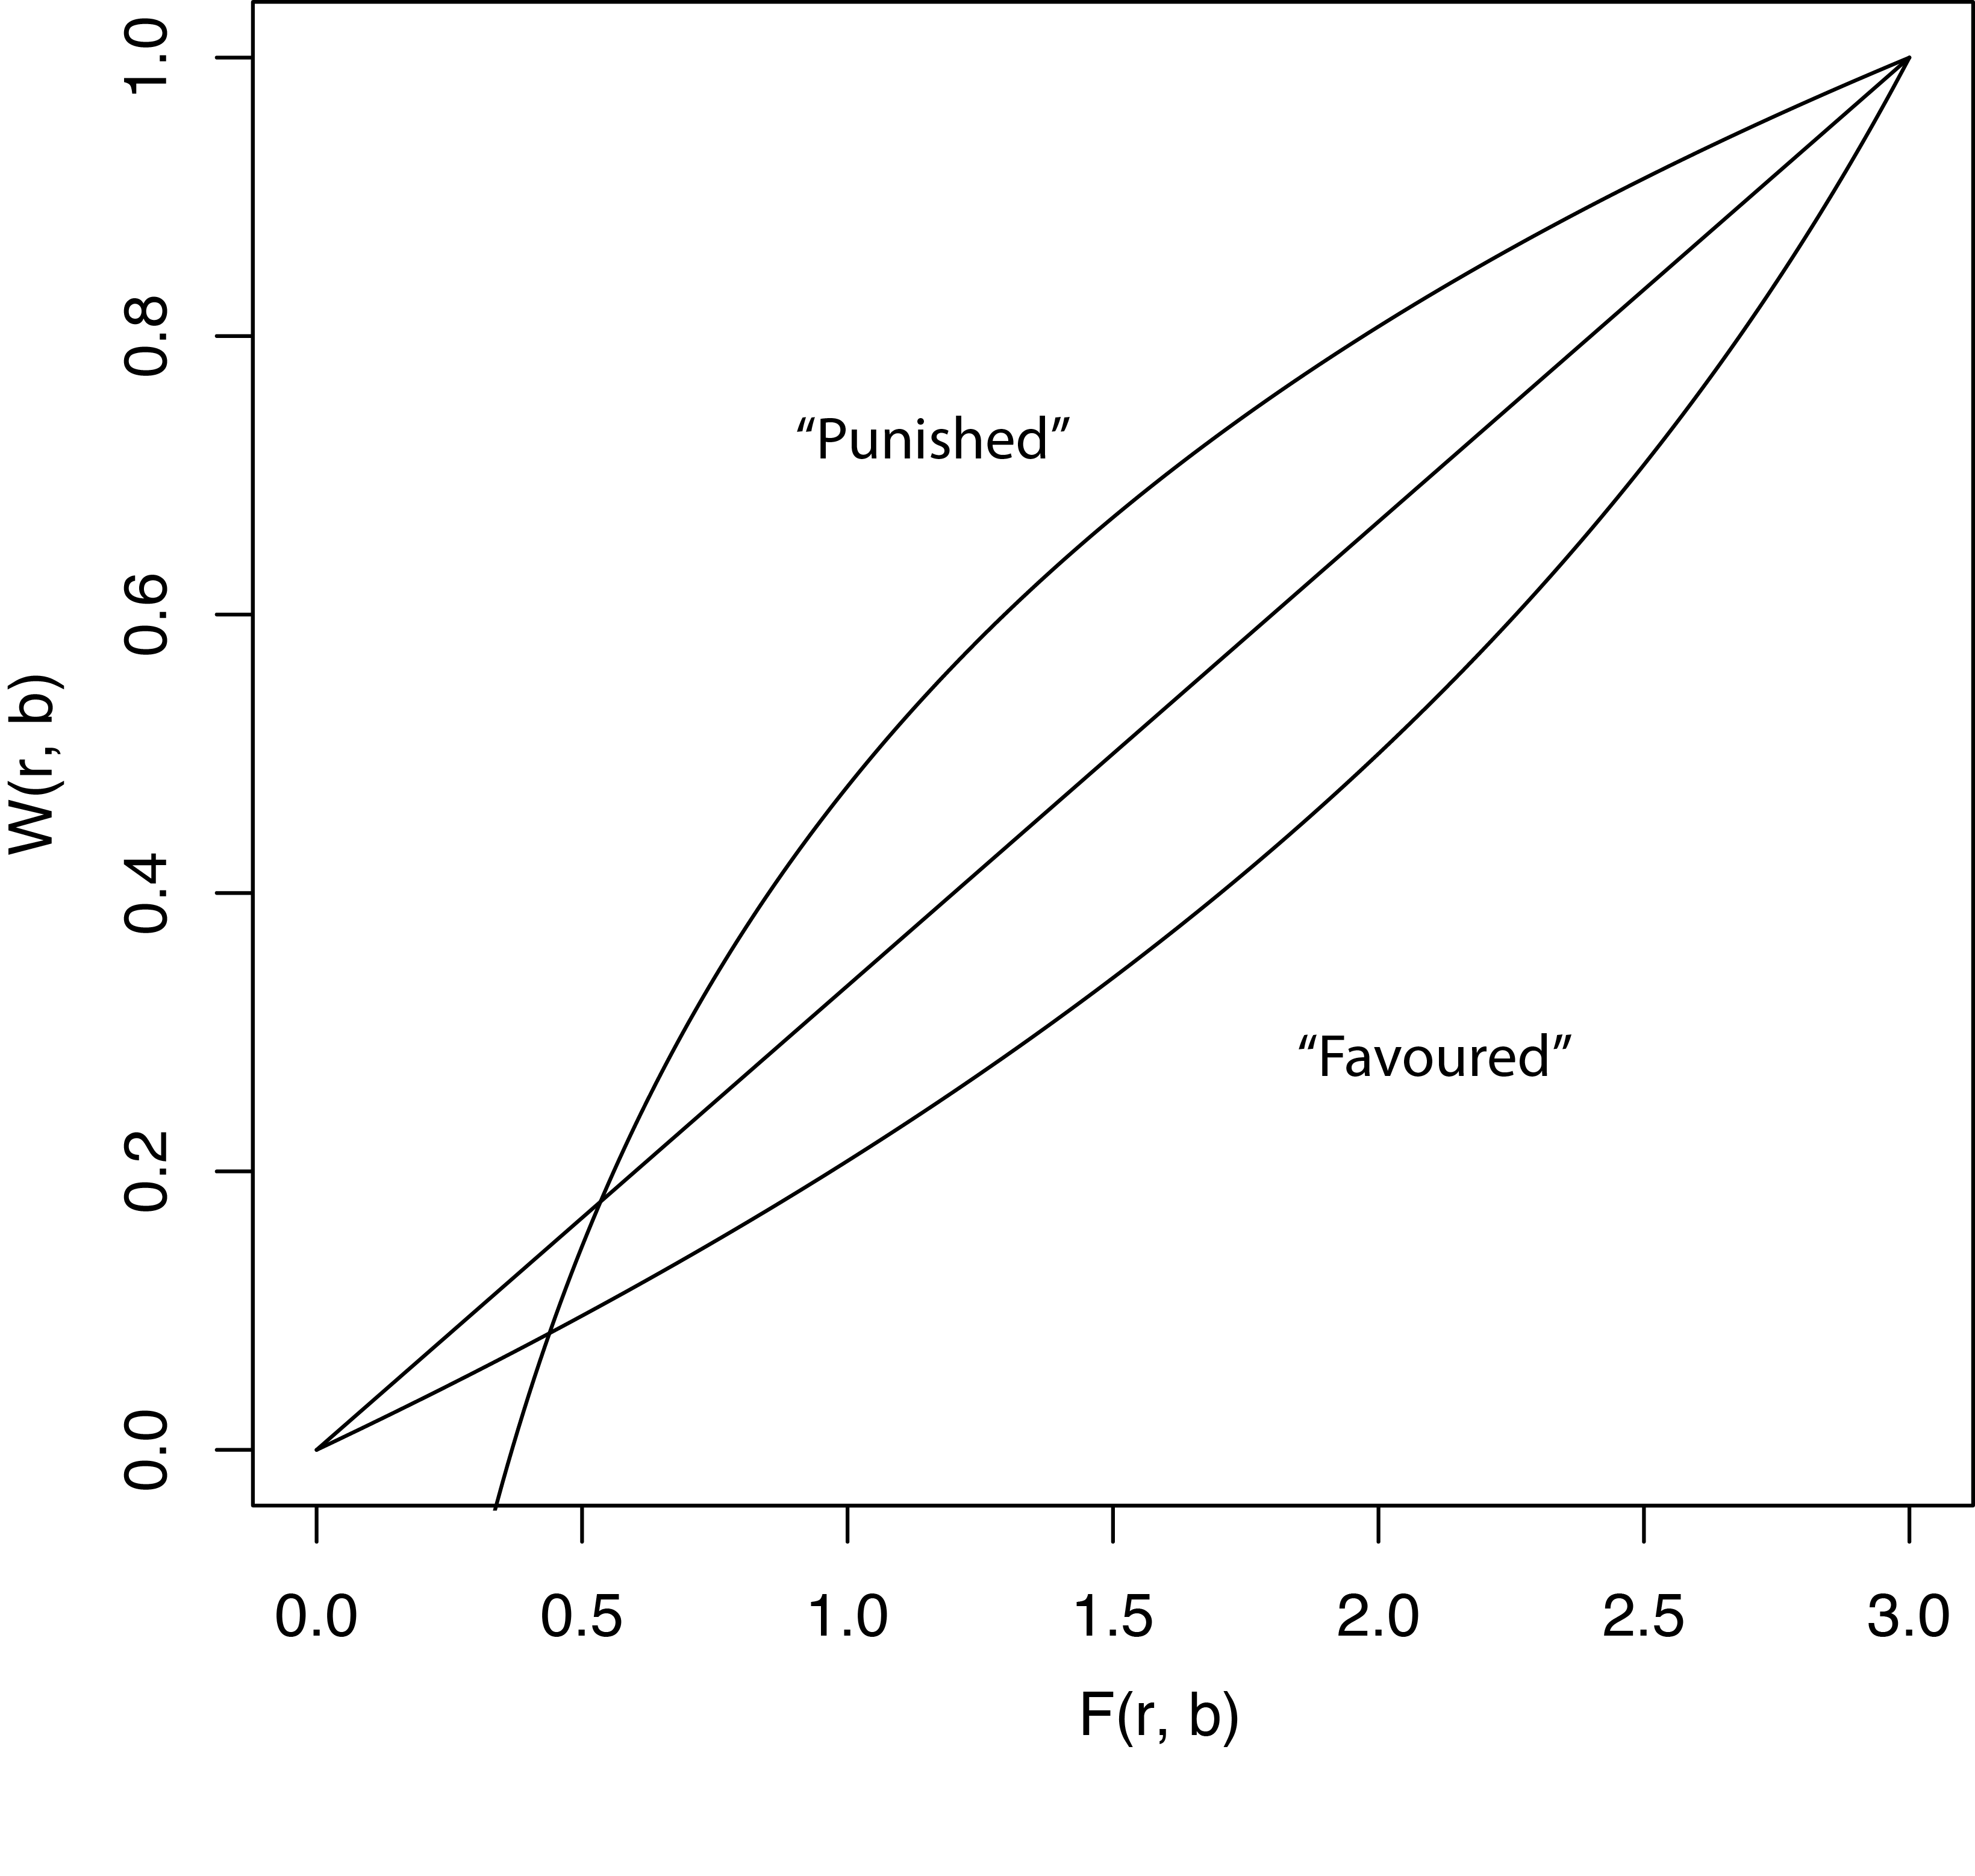
\includegraphics[width=0.3 \textwidth]{fig12/weight_functions.png}
  \caption{Two different weight functions)}
\end{figure}

%
% Treating gaps
%
\subsubsection*{Treating gaps}
Position-specific gap penalties are usually added to profiles.

\bigskip 

%\end{document}
